\section{Latex Examples - Temp} 

Chapter introduction

\subsection{Section 1}
\label{sec:sec-1}

Citation ~\cite{s:source1}.

Reference to section 1: \ref{sec:sec-1}

\begin{table}[h]
\centering
\caption{Energy use in the US food system as a percentage of total domestic energy}
\label{tab_agric_energy}

\vspace{6pt}
\begin{tabular}{lcccc}
\toprule
Process & \multicolumn{3}{c}{Study} & Average \\
\cmidrule(r){2-4}
 & Fluck & Singh & Poincelot & \\
\midrule
Production & 55.36  & 62.86 & 62.86 & 60.36 \\
Wholesale/Retail & 28.93    & 28.21 & 9.29  & 22.14 \\
Transport & 46.43   & 8.57  & 28.21 & 27.74 \\
\midrule
\midrule
Total domestic energy (\%) & 4.51   & 4.62  & 4.76  & 4.63 \\
\bottomrule
\end{tabular}
\end{table}

Table \ref{tab_agric_energy} reference.

\subsection{Section 2}
\label{sec:sec-2}

Descriptions:

\begin{description}

\item[Item 1]
Descript

\item[Item]
asdf. Cite 2 ~\cite{s:source2}

\end{description}

\subsection{Section 3}

asdf

\subsubsection{Sub section}

Some more stuff

\begin{figure}[h]
    \centering
    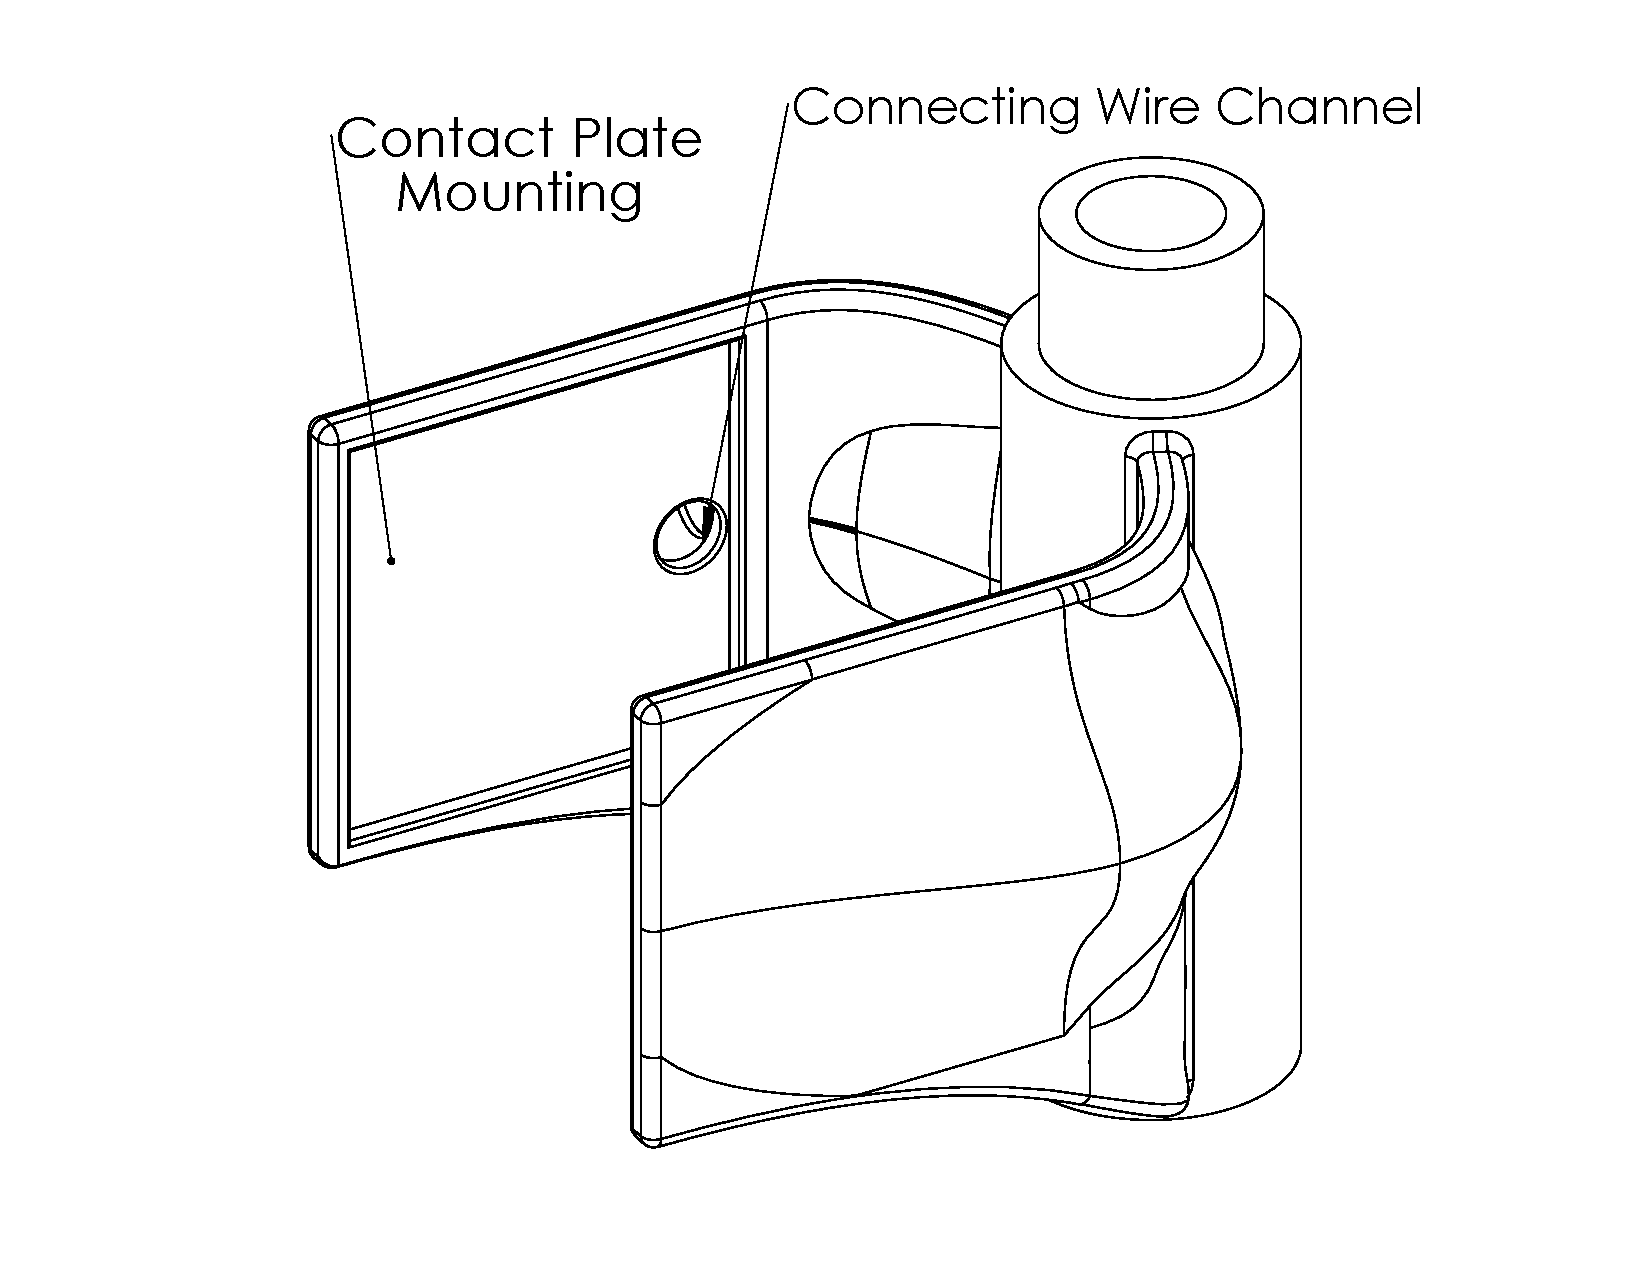
\includegraphics[width=.5\textwidth]{images/MoistureSensor}
    \caption{Custom Moisture Sensor}
    \label{fig:moistureSensor}
\end{figure}

And to reference figure \ref{fig:moistureSensor}

\subsection{Equations}

To reference the equation: \ref{eq:syseq2}

\begin{equation}
	\label{eq:syseq2}
	\dot{x_2} = f_2 = {\frac {u}{0.000105\,m\,\left(x_1 + 6.2 \right) ^{4}}} - 9.81
\end{equation}


\begin{align}
	\label{eq:fderivA}
	 {\frac {df_1}{dx_1}} &= 0 &  {\frac {df_1}{dx_2}} &=1 &  {\frac {df_2}{dx_1}} &= - \,{\frac {38095.23810\,u}{m\left( x_1 + 6.2 \right) ^{5}}} &  {\frac {df_2}{dx_2}} &=0
\end{align}


\begin{equation}
	\label{eq:finalLinearizedx}
	{\bf \dot{\lambda}} - {\bf \dot{\lambda}^\star} = 
	\left[
		\begin{array}{cc}
			 0 & 1 \\
			 -{\frac {39.24}{z_0 + 6.2}} & 0 \\
		\end{array}
	\right]
	\left(
		{\bf x} - {\bf x^\star}
	\right)
	+ 
	\left[
		\begin{array}{c}
			 0 \\
			{\frac {9523.809524}{m\,\left( z_0 + 6.2 \right) ^{4}}} \\
		\end{array}
	\right]
	\left(
		u - u^\star
	\right)S
\end{equation}
